\documentclass[12pt, a4paper]{report}

% ── Packages ──────────────────────────────────────────────────────────────────
\usepackage[utf8]{inputenc}
\usepackage[T1]{fontenc}
\usepackage{lmodern}
\usepackage[margin=1in]{geometry}
\usepackage{graphicx}
\usepackage{xcolor}
\usepackage{tikz}
\usetikzlibrary{positioning, arrows.meta, calc, decorations.pathreplacing, shapes.multipart}
\usepackage{listings}
\usepackage{hyperref}
\usepackage{booktabs}
\usepackage{tabularx}
\usepackage{caption}
\usepackage{fancyhdr}
\usepackage{titlesec}
\usepackage{enumitem}
\usepackage{amsmath}

% ── Colors ────────────────────────────────────────────────────────────────────
\definecolor{proto-blue}{HTML}{2563EB}
\definecolor{proto-dark}{HTML}{1E293B}
\definecolor{proto-gray}{HTML}{64748B}
\definecolor{proto-light}{HTML}{F1F5F9}
\definecolor{proto-green}{HTML}{059669}
\definecolor{proto-red}{HTML}{DC2626}
\definecolor{proto-orange}{HTML}{D97706}
\definecolor{code-bg}{HTML}{F8FAFC}

% ── Hyperref ──────────────────────────────────────────────────────────────────
\hypersetup{
    colorlinks=true,
    linkcolor=proto-blue,
    urlcolor=proto-blue,
    citecolor=proto-green,
}

% ── Code listings ─────────────────────────────────────────────────────────────
\lstdefinestyle{protoc}{
    language=C,
    basicstyle=\ttfamily\small,
    backgroundcolor=\color{code-bg},
    keywordstyle=\color{proto-blue}\bfseries,
    commentstyle=\color{proto-gray}\itshape,
    stringstyle=\color{proto-green},
    numberstyle=\tiny\color{proto-gray},
    numbers=left,
    numbersep=8pt,
    frame=single,
    rulecolor=\color{proto-gray!30},
    breaklines=true,
    tabsize=4,
    showstringspaces=false,
    xleftmargin=1.5em,
    framexleftmargin=1em,
}
\lstset{style=protoc}

% ── Headers ───────────────────────────────────────────────────────────────────
\pagestyle{fancy}
\fancyhf{}
\fancyhead[L]{\small\textcolor{proto-gray}{ProtoDB}}
\fancyhead[R]{\small\textcolor{proto-gray}{\leftmark}}
\fancyfoot[C]{\small\textcolor{proto-gray}{\thepage}}
\renewcommand{\headrulewidth}{0.4pt}

% ── Title formatting ─────────────────────────────────────────────────────────
\titleformat{\chapter}[display]
    {\normalfont\Huge\bfseries\color{proto-dark}}
    {\textcolor{proto-blue}{\chaptertitlename\ \thechapter}}{20pt}{\Huge}
\titleformat{\section}
    {\normalfont\Large\bfseries\color{proto-dark}}{{\textcolor{proto-blue}{\thesection}}}{1em}{}
\titleformat{\subsection}
    {\normalfont\large\bfseries\color{proto-dark}}{{\textcolor{proto-blue}{\thesubsection}}}{1em}{}

% ── Document ──────────────────────────────────────────────────────────────────
\begin{document}

% ── Title Page ────────────────────────────────────────────────────────────────
\begin{titlepage}
    \centering
    \vspace*{3cm}

    {\Huge\bfseries\textcolor{proto-dark}{ProtoDB}\par}
    \vspace{0.5cm}
    {\Large\textcolor{proto-gray}{Building a Database from Scratch}\par}

    \vspace{2cm}

    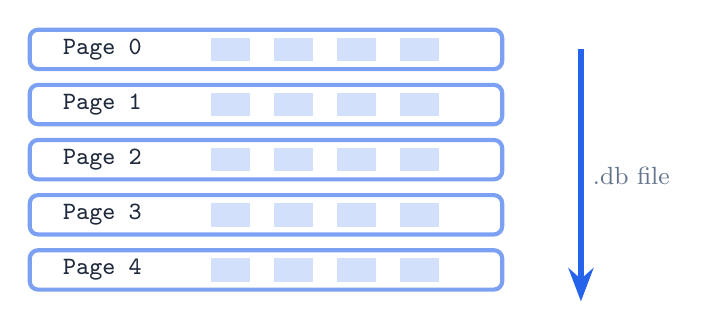
\begin{tikzpicture}
        \foreach \i in {0,...,4} {
            \draw[proto-blue!60, line width=1.5pt, rounded corners=3pt]
                (0, -\i*0.7) rectangle (6, -\i*0.7 - 0.5);
            \node[anchor=west, font=\ttfamily\small, text=proto-dark]
                at (0.3, -\i*0.7 - 0.25) {Page \i};
            \foreach \j in {1,...,4} {
                \fill[proto-blue!20] (1.5+\j*0.8, -\i*0.7 - 0.1) rectangle (1.5+\j*0.8+0.5, -\i*0.7 - 0.4);
            }
        }
        \draw[proto-blue, line width=2pt, -Stealth] (7, -0.25) -- (7, -3.45)
            node[midway, right, font=\small, text=proto-gray] {.db file};
    \end{tikzpicture}

    \vfill

    {\large Omar\par}
    \vspace{0.3cm}
    {\textcolor{proto-gray}{\today}\par}
\end{titlepage}

\tableofcontents
\newpage


% ══════════════════════════════════════════════════════════════════════════════
\chapter{Motivation}
% ══════════════════════════════════════════════════════════════════════════════

Honestly, this project exists because I wanted to see if I actually understood
what I'd been reading and watching, or if I was just nodding along.

I spent a good amount of time going through Andy Pavlo's CMU 15-445 lectures
on database systems\footnote{\url{https://15445.courses.cs.cmu.edu/}} and
reading Alex Petrov's \textit{Database Internals}\footnote{Petrov, A.
\textit{Database Internals: A Deep Dive into How Distributed Data Systems
Work}. O'Reilly Media, 2019.}. Both are fantastic resources---the lectures
give you the systems thinking and the book fills in the gaps with how things
are actually laid out on disk, how storage engines manage pages, what a buffer
pool is really doing under the hood, and so on.

But there's a difference between understanding a concept when someone explains
it on a whiteboard and actually writing the code that makes it work. The edge
cases, the off-by-one errors in your slot directory, the moment you realize
your free list is corrupting page 0---that's where the real learning happens.

So ProtoDB is not trying to be the next PostgreSQL. It's not trying to be
production-ready or feature-complete. It's just me, writing C, messing up,
fixing it, and hopefully coming out the other side with a much better grasp
of how databases actually work at the lowest level.

The plan is to build things layer by layer:
\begin{enumerate}[itemsep=2pt]
    \item Pages and disk I/O
    \item Buffer pool manager with page eviction
    \item Vector indexing (flat scan, then HNSW)
    \item Heap file organization
    \item B-tree indexing
    \item A simple query execution layer
\end{enumerate}

Each chapter in this document corresponds to one of those layers. I'll try to
document not just what I built, but \textit{why} I made the choices I did,
what the tradeoffs are, and where I got the ideas from. Partly so future-me
can remember, and partly because writing things down forces you to actually
understand them.

Let's start with pages.


% ══════════════════════════════════════════════════════════════════════════════
\chapter{Storage Manager}
% ══════════════════════════════════════════════════════════════════════════════

The storage manager is the lowest layer of the system. It owns the database
file on disk and provides the rest of the engine with a simple abstraction:
\textit{read page N, write page N, give me a new page, free this page}. Every
byte of user data flows through here.

This chapter covers the two components that make up this layer: the
\textbf{slotted page} format (how data is organized inside a single 8 KB
page) and the \textbf{storage manager} itself (how pages are persisted to a
\texttt{.db} file).


% ── 2.1 Architecture ─────────────────────────────────────────────────────────
\section{Architecture Overview}

The storage layer is split into two files with distinct responsibilities:

\begin{center}
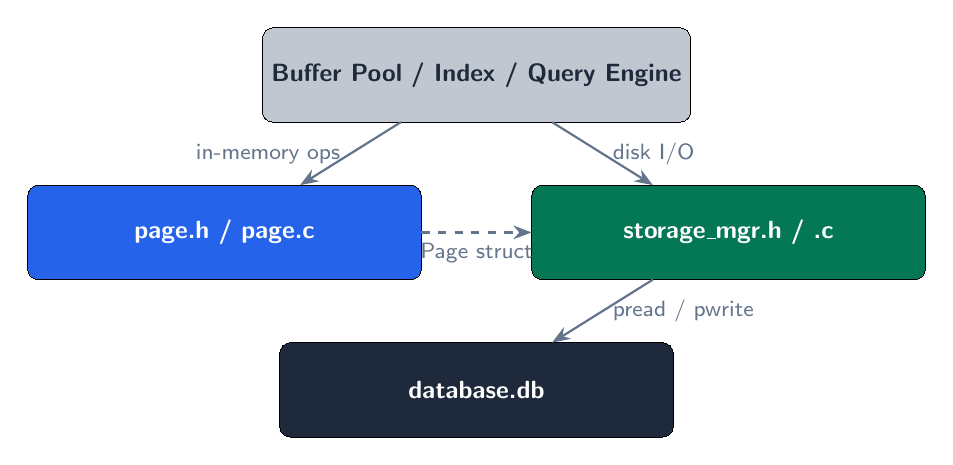
\begin{tikzpicture}[
    box/.style={draw, rounded corners=4pt, minimum width=5cm, minimum height=1.2cm,
                text=white, font=\sffamily\small\bfseries, line width=0},
    arr/.style={-Stealth, thick, proto-gray},
    lbl/.style={font=\sffamily\footnotesize, text=proto-gray},
]
    % Upper layers
    \node[box, fill=proto-gray!40, text=proto-dark] (upper) at (0, 4) {Buffer Pool / Index / Query Engine};

    % Page API
    \node[box, fill=proto-blue] (page) at (-3.2, 2) {page.h / page.c};
    \node[box, fill=proto-green!80!black] (storage) at (3.2, 2) {storage\_mgr.h / .c};

    % Disk
    \node[box, fill=proto-dark] (disk) at (0, 0) {database.db};

    % Arrows
    \draw[arr] (upper) -- (page) node[midway, left, lbl] {in-memory ops};
    \draw[arr] (upper) -- (storage) node[midway, right, lbl] {disk I/O};
    \draw[arr] (storage) -- (disk) node[midway, right, lbl] {pread / pwrite};
    \draw[arr, dashed] (page) -- (storage) node[midway, below, lbl] {Page struct};

\end{tikzpicture}
\end{center}

\begin{itemize}[itemsep=4pt]
    \item \textbf{page.c} --- Operates on in-memory page buffers. Knows nothing
          about files or disk. Given a \texttt{Page} struct, it can insert,
          read, delete, update, and compact records within that page's
          \texttt{data[8192]} array.
    \item \textbf{storage\_mgr.c} --- Owns the file descriptor. Reads and
          writes raw 8 KB blocks between memory and the \texttt{.db} file.
          Manages the meta page (page 0) and the free page list.
\end{itemize}

This separation is intentional. The page code is pure memory manipulation with
no system calls, which makes it easy to test in isolation. The storage manager
handles all the messy POSIX I/O. This mirrors the design described in CMU
15-445 Lecture 3 (Database Storage I)\footnote{%
\url{https://15445.courses.cs.cmu.edu/fall2024/slides/03-storage1.pdf}}.


% ── 2.2 Page Layout ──────────────────────────────────────────────────────────
\section{Slotted Page Layout}

Each page is a fixed 8192-byte block (8 KB). Internally it uses the \textbf{slotted
page} format, which is the same approach used by PostgreSQL, SQLite, and most
disk-oriented databases\footnote{Ramakrishnan, R. \& Gehrke, J. \textit{%
Database Management Systems}, 3rd ed. Chapter 9.6 --- Page Formats.}.

\begin{center}
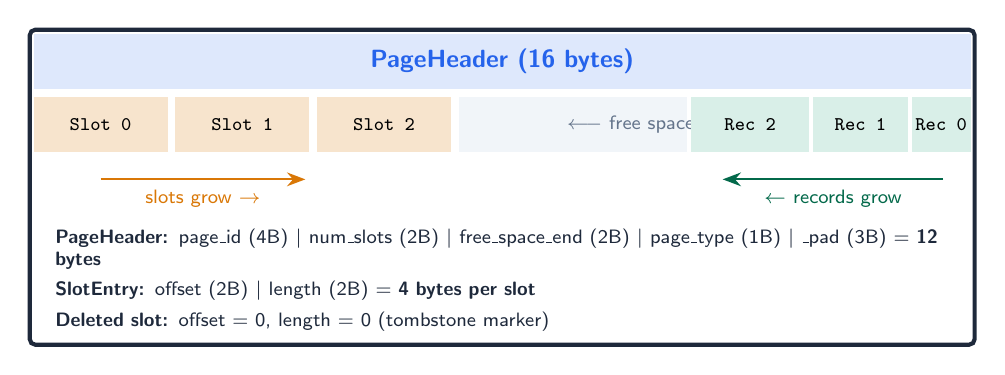
\begin{tikzpicture}[
    cell/.style={draw, minimum height=0.8cm, font=\ttfamily\scriptsize, anchor=west},
    brace/.style={decorate, decoration={brace, amplitude=6pt, raise=2pt}},
]
    \def\pw{12}
    \def\ph{0.8}

    % Page outline
    \draw[proto-dark, line width=1.5pt, rounded corners=2pt] (0,0) rectangle (\pw, -5*\ph);

    % Header
    \fill[proto-blue!15] (0.05, -0.05) rectangle (\pw-0.05, -\ph+0.05);
    \node[font=\sffamily\small\bfseries, text=proto-blue] at (\pw/2, -\ph/2)
        {PageHeader (16 bytes)};

    % Slot array
    \foreach \i/\label in {0/Slot 0, 1/Slot 1, 2/Slot 2} {
        \fill[proto-orange!20] (0.05+\i*1.8, -\ph-0.05) rectangle (0.05+\i*1.8+1.7, -2*\ph+0.05);
        \node[font=\ttfamily\scriptsize] at (0.05+\i*1.8+0.85, -1.5*\ph) {\label};
    }

    % Free space
    \fill[proto-light] (5.45, -\ph-0.05) rectangle (\pw-3.65, -2*\ph+0.05);
    \node[font=\sffamily\scriptsize, text=proto-gray] at (7.9, -1.5*\ph) {$\longleftarrow$ free space $\longrightarrow$};

    % Records (growing from right)
    \fill[proto-green!15] (\pw-3.6, -\ph-0.05) rectangle (\pw-2.1, -2*\ph+0.05);
    \node[font=\ttfamily\scriptsize] at (\pw-2.85, -1.5*\ph) {Rec 2};

    \fill[proto-green!15] (\pw-2.05, -\ph-0.05) rectangle (\pw-0.85, -2*\ph+0.05);
    \node[font=\ttfamily\scriptsize] at (\pw-1.45, -1.5*\ph) {Rec 1};

    \fill[proto-green!15] (\pw-0.8, -\ph-0.05) rectangle (\pw-0.05, -2*\ph+0.05);
    \node[font=\ttfamily\scriptsize] at (\pw-0.425, -1.5*\ph) {Rec 0};

    % Arrows
    \draw[proto-orange, -Stealth, thick] (0.9, -2*\ph-0.3) -- (3.5, -2*\ph-0.3)
        node[midway, below, font=\sffamily\scriptsize] {slots grow $\rightarrow$};
    \draw[proto-green!70!black, -Stealth, thick] (\pw-0.4, -2*\ph-0.3) -- (\pw-3.2, -2*\ph-0.3)
        node[midway, below, font=\sffamily\scriptsize] {$\leftarrow$ records grow};

    % Details box
    \node[anchor=north west, font=\sffamily\scriptsize, text=proto-dark,
          text width=11.5cm] at (0.2, -3*\ph) {
        \textbf{PageHeader:} page\_id (4B) $\mid$ num\_slots (2B) $\mid$
        free\_space\_end (2B) $\mid$ page\_type (1B) $\mid$ \_pad (3B) = \textbf{12 bytes}\\[3pt]
        \textbf{SlotEntry:} offset (2B) $\mid$ length (2B) = \textbf{4 bytes per slot}\\[3pt]
        \textbf{Deleted slot:} offset = 0, length = 0 (tombstone marker)
    };

\end{tikzpicture}
\end{center}

\subsection{Why Slotted Pages?}

\begin{table}[h]
\centering
\begin{tabularx}{\textwidth}{lXX}
\toprule
\textbf{Approach} & \textbf{Advantage} & \textbf{Disadvantage} \\
\midrule
Fixed-length records &
    Simple offset math, O(1) access &
    Wastes space for variable-length data \\
\addlinespace
Log-structured (append-only) &
    Sequential writes, great for SSDs &
    Reads require index, compaction is expensive \\
\addlinespace
\textbf{Slotted page} &
    Variable-length records, stable slot IDs,
    records can move during compaction without
    breaking external references &
    Slightly more bookkeeping per page \\
\bottomrule
\end{tabularx}
\caption{Comparison of page organization strategies}
\end{table}

The slotted page is the standard choice for a disk-oriented DBMS that needs to
support variable-length records. The indirection through the slot array is the
key insight: higher layers reference records by \texttt{(page\_id, slot\_index)},
and the page is free to physically rearrange records internally (e.g., during
compaction) without invalidating those references\footnote{This design is
discussed in detail in Ramakrishnan \& Gehrke Ch. 9.6 and demonstrated in CMU
15-445 Project 1.}.


\subsection{Implementation Choices}

\subsubsection{Slot Reuse}

When a record is deleted, its \texttt{SlotEntry} is zeroed out
(\texttt{offset = 0, length = 0}) rather than removed from the array. On the
next insert, the slot array is scanned for a dead slot before appending a new
one.

\begin{table}[h]
\centering
\begin{tabularx}{\textwidth}{lXX}
\toprule
& \textbf{Our approach (scan for dead slot)} & \textbf{Alternative (always append)} \\
\midrule
\textbf{Pro} &
    Slot array doesn't grow unboundedly for insert-heavy workloads with deletes &
    O(1) insert, no scan needed \\
\addlinespace
\textbf{Con} &
    O(n) scan on insert, where n = num\_slots &
    Slot array can waste significant space over time \\
\bottomrule
\end{tabularx}
\caption{Slot reuse tradeoff}
\end{table}

The scan cost is negligible in practice because \texttt{num\_slots} is bounded
by what fits in an 8 KB page. With 4-byte slots and a 12-byte header, the
absolute maximum is around 1021 slots---and real records are much larger than
zero bytes, so the actual count is far smaller.


\subsubsection{In-Place Update Fast Path}

\texttt{page\_update\_record} checks whether the new record is the same length
as the old one. If so, it does a direct \texttt{memcpy} over the existing data
without touching the slot directory or free space pointer.

\begin{lstlisting}
if (len == s->length) {
    memcpy(p->data + s->offset, data, len);
    return 0;
}
\end{lstlisting}

This avoids unnecessary compaction for the common case of fixed-schema updates
(e.g., updating an integer column).

For different-length updates, the function deletes the old record, attempts
insertion, and triggers compaction if the contiguous free gap is too small but
reclaimable space exists.


\subsubsection{Compaction Strategy}

\texttt{page\_compact} walks the slot array in order and repacks all live
records contiguously toward the high end of the page, using \texttt{memmove}
to handle overlapping regions safely.

\begin{center}
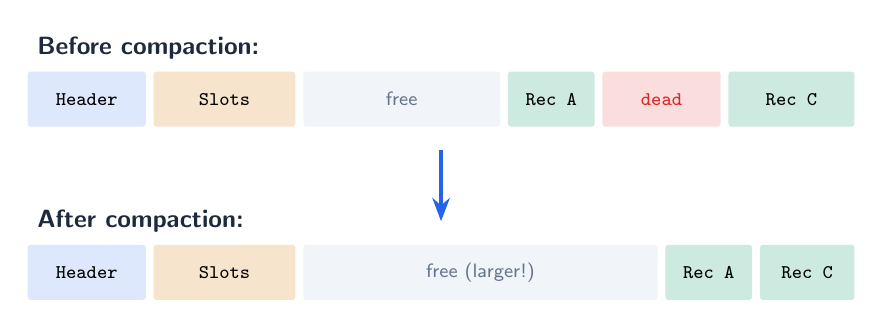
\begin{tikzpicture}[
    block/.style={draw, minimum height=0.7cm, font=\ttfamily\scriptsize, rounded corners=1pt},
]
    % Before
    \node[font=\sffamily\small\bfseries, text=proto-dark, anchor=west] at (0, 1) {Before compaction:};

    \fill[proto-blue!15, rounded corners=1pt] (0, 0) rectangle (1.5, 0.7);
    \node[font=\ttfamily\scriptsize] at (0.75, 0.35) {Header};

    \fill[proto-orange!20, rounded corners=1pt] (1.6, 0) rectangle (3.4, 0.7);
    \node[font=\ttfamily\scriptsize] at (2.5, 0.35) {Slots};

    \fill[proto-light, rounded corners=1pt] (3.5, 0) rectangle (6, 0.7);
    \node[font=\sffamily\scriptsize, text=proto-gray] at (4.75, 0.35) {free};

    \fill[proto-green!20, rounded corners=1pt] (6.1, 0) rectangle (7.2, 0.7);
    \node[font=\ttfamily\scriptsize] at (6.65, 0.35) {Rec A};

    \fill[proto-red!15, rounded corners=1pt] (7.3, 0) rectangle (8.8, 0.7);
    \node[font=\ttfamily\scriptsize, text=proto-red] at (8.05, 0.35) {dead};

    \fill[proto-green!20, rounded corners=1pt] (8.9, 0) rectangle (10.5, 0.7);
    \node[font=\ttfamily\scriptsize] at (9.7, 0.35) {Rec C};

    % After
    \node[font=\sffamily\small\bfseries, text=proto-dark, anchor=west] at (0, -1.2) {After compaction:};

    \fill[proto-blue!15, rounded corners=1pt] (0, -2.2) rectangle (1.5, -1.5);
    \node[font=\ttfamily\scriptsize] at (0.75, -1.85) {Header};

    \fill[proto-orange!20, rounded corners=1pt] (1.6, -2.2) rectangle (3.4, -1.5);
    \node[font=\ttfamily\scriptsize] at (2.5, -1.85) {Slots};

    \fill[proto-light, rounded corners=1pt] (3.5, -2.2) rectangle (8, -1.5);
    \node[font=\sffamily\scriptsize, text=proto-gray] at (5.75, -1.85) {free (larger!)};

    \fill[proto-green!20, rounded corners=1pt] (8.1, -2.2) rectangle (9.2, -1.5);
    \node[font=\ttfamily\scriptsize] at (8.65, -1.85) {Rec A};

    \fill[proto-green!20, rounded corners=1pt] (9.3, -2.2) rectangle (10.5, -1.5);
    \node[font=\ttfamily\scriptsize] at (9.9, -1.85) {Rec C};

    % Arrow
    \draw[proto-blue, -Stealth, very thick] (5.25, -0.3) -- (5.25, -1.2);
\end{tikzpicture}
\end{center}

Compaction is \textbf{not} triggered automatically on delete. It only runs
when \texttt{page\_update\_record} needs more contiguous space than the gap
provides. This is a deliberate choice:

\begin{itemize}[itemsep=2pt]
    \item Deletes stay O(1)---just zero two bytes.
    \item Compaction is O(n) in the number of live records, so we defer it
          until actually needed.
    \item This matches the approach described in Petrov's \textit{Database
          Internals}, Chapter 3 (File Formats), where compaction is treated as
          a maintenance operation rather than an inline cost\footnote{Petrov,
          A. \textit{Database Internals}, Ch. 3: File Formats, section on
          slotted pages and garbage collection.}.
\end{itemize}


% ── 2.3 Storage Manager ──────────────────────────────────────────────────────
\section{Storage Manager}

The storage manager (\texttt{storage\_mgr.c}) is the interface between
in-memory pages and the \texttt{.db} file on disk. Its API is intentionally
minimal:

\begin{lstlisting}
int       storage_open(StorageManager *sm, const char *path);
int       storage_close(StorageManager *sm);
int       storage_read_page(StorageManager *sm, page_id_t id, Page *p);
int       storage_write_page(StorageManager *sm, page_id_t id, Page *p);
int       storage_allocate_page(StorageManager *sm, page_id_t *out);
int       storage_deallocate_page(StorageManager *sm, page_id_t id);
page_id_t storage_num_pages(StorageManager *sm);
\end{lstlisting}


\subsection{File Layout}

The \texttt{.db} file is a flat sequence of 8 KB pages. Page $N$ lives at
byte offset $N \times 8192$.

\begin{center}
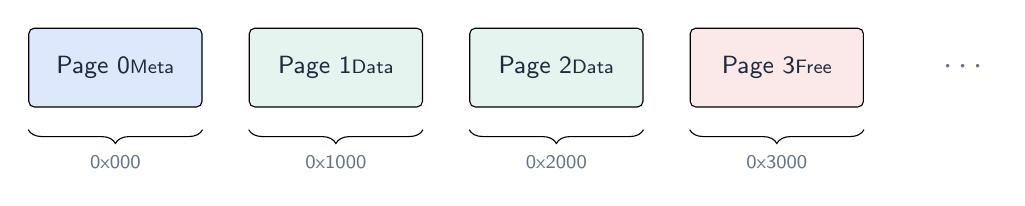
\begin{tikzpicture}[
    pg/.style={draw, minimum width=2.2cm, minimum height=1cm,
               rounded corners=2pt, font=\sffamily\small},
]
    \node[pg, fill=proto-blue!15, text=proto-dark] (p0) at (0,0) {Page 0\\[-2pt]{\scriptsize Meta}};
    \node[pg, fill=proto-green!10, text=proto-dark] (p1) at (2.8,0) {Page 1\\[-2pt]{\scriptsize Data}};
    \node[pg, fill=proto-green!10, text=proto-dark] (p2) at (5.6,0) {Page 2\\[-2pt]{\scriptsize Data}};
    \node[pg, fill=proto-red!10, text=proto-dark] (p3) at (8.4,0) {Page 3\\[-2pt]{\scriptsize Free}};
    \node[font=\sffamily\large, text=proto-gray] at (10.8, 0) {$\cdots$};

    \draw[decorate, decoration={brace, amplitude=5pt, mirror, raise=8pt}]
        (p0.south west) -- (p0.south east)
        node[midway, below=14pt, font=\sffamily\scriptsize, text=proto-gray] {0x000};
    \draw[decorate, decoration={brace, amplitude=5pt, mirror, raise=8pt}]
        (p1.south west) -- (p1.south east)
        node[midway, below=14pt, font=\sffamily\scriptsize, text=proto-gray] {0x1000};
    \draw[decorate, decoration={brace, amplitude=5pt, mirror, raise=8pt}]
        (p2.south west) -- (p2.south east)
        node[midway, below=14pt, font=\sffamily\scriptsize, text=proto-gray] {0x2000};
    \draw[decorate, decoration={brace, amplitude=5pt, mirror, raise=8pt}]
        (p3.south west) -- (p3.south east)
        node[midway, below=14pt, font=\sffamily\scriptsize, text=proto-gray] {0x3000};
\end{tikzpicture}
\end{center}


\subsection{Meta Page (Page 0)}

Page 0 is special. It stores the \texttt{MetaPageHeader} at offset
\texttt{PAGE\_DATA\_OFFSET} inside the page's data buffer:

\begin{lstlisting}
typedef struct {
    uint32_t   magic;           // 0xDB1234
    uint32_t   schema_version;  // currently 1
    page_id_t  page_count;      // total pages in the file
    page_id_t  free_list_head;  // first free page, or INVALID_PAGE_ID
} MetaPageHeader;
\end{lstlisting}

The magic number serves two purposes:
\begin{enumerate}[itemsep=2pt]
    \item \textbf{File identification} --- on open, we read page 0 and verify
          the magic. If it doesn't match, we reject the file rather than
          silently corrupting someone's data.
    \item \textbf{Endianness detection} --- if we ever need to support
          cross-architecture portability, the magic number reveals the byte
          order of the file.
\end{enumerate}

This pattern is standard across database implementations. SQLite uses
\texttt{"SQLite format 3\textbackslash000"} as its header
string\footnote{\url{https://www.sqlite.org/fileformat.html}}, and
InnoDB uses a similar magic-based validation on tablespace files.


\subsection{I/O: pread and pwrite}

All disk I/O uses \texttt{pread(2)} and \texttt{pwrite(2)} instead of the
more common \texttt{read}/\texttt{write} + \texttt{lseek} combination.

\begin{table}[h]
\centering
\begin{tabularx}{\textwidth}{lXX}
\toprule
\textbf{Approach} & \textbf{Pro} & \textbf{Con} \\
\midrule
\texttt{lseek} + \texttt{read/write} &
    Works everywhere, simple mental model &
    Not thread-safe without a mutex: two threads can interleave
    \texttt{lseek} and \texttt{read} on the same fd \\
\addlinespace
\textbf{\texttt{pread} / \texttt{pwrite}} &
    Atomic seek+read in one syscall, inherently thread-safe,
    no shared file offset to corrupt &
    POSIX-only (not available on Windows without \texttt{ReadFile} wrapper) \\
\addlinespace
\texttt{mmap} &
    Zero-copy, OS manages caching, simple random access &
    OS controls eviction (fights with buffer pool), TLB shootdowns on
    multicore, hard to handle I/O errors, SIGBUS risk \\
\bottomrule
\end{tabularx}
\caption{Disk I/O strategy comparison}
\end{table}

We chose \texttt{pread}/\texttt{pwrite} because they give us explicit control
over I/O (important when we build the buffer pool later) while being naturally
thread-safe. The \texttt{mmap} approach, while tempting, is explicitly
discouraged by Andy Pavlo in the CMU 15-445 course---and backed by the paper
\textit{``Are You Sure You Want to Use MMAP in Your Database Management
System?''}\footnote{Crotty, A. et al., \textit{Are You Sure You Want to Use
MMAP in Your DBMS?}, CIDR 2022. \url{https://db.cs.cmu.edu/mmap-cidr2022/}}.


\subsection{Page Allocation}

\texttt{storage\_allocate\_page} either pops a page from the free list or
extends the file:

\begin{center}
\begin{tikzpicture}[
    node distance=1.2cm,
    decision/.style={diamond, draw, fill=proto-blue!10, text=proto-dark,
                     font=\sffamily\scriptsize, aspect=2.5, inner sep=1pt},
    process/.style={draw, rounded corners=3pt, fill=proto-green!10, text=proto-dark,
                    font=\sffamily\scriptsize, minimum width=3cm, minimum height=0.7cm},
    arr/.style={-Stealth, thick, proto-gray},
]
    \node[process] (start) {allocate\_page() called};
    \node[decision, below=of start] (check) {free\_list\_head !=\\INVALID?};
    \node[process, below left=1.2cm and 1.5cm of check] (pop) {Pop head from free list\\Read next-pointer from page\\Update meta};
    \node[process, below right=1.2cm and 1.5cm of check] (extend) {Increment page\_count\\ftruncate() to extend file\\Write empty page};
    \node[process, below=2.5cm of check] (done) {Return new page\_id};

    \draw[arr] (start) -- (check);
    \draw[arr] (check) -| node[near start, above, font=\sffamily\scriptsize] {yes} (pop);
    \draw[arr] (check) -| node[near start, above, font=\sffamily\scriptsize] {no} (extend);
    \draw[arr] (pop) |- (done);
    \draw[arr] (extend) |- (done);
\end{tikzpicture}
\end{center}


\subsection{Free List Design}

Deallocated pages form a singly-linked list threaded through the pages
themselves. When a page is freed:

\begin{enumerate}[itemsep=2pt]
    \item The page is zeroed and its type set to \texttt{PAGE\_TYPE\_FREE}.
    \item The current \texttt{free\_list\_head} is written into the page's
          data at \texttt{PAGE\_DATA\_OFFSET} (the first 4 bytes after the
          header).
    \item \texttt{free\_list\_head} is updated to point to this page.
    \item The meta page is flushed to disk.
\end{enumerate}

\begin{center}
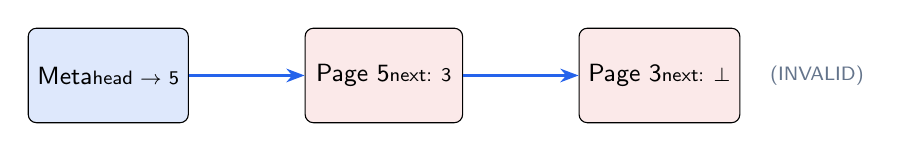
\begin{tikzpicture}[
    pg/.style={draw, rounded corners=3pt, minimum width=2cm, minimum height=1.2cm,
               font=\sffamily\small},
    arr/.style={-Stealth, thick, proto-blue},
]
    \node[pg, fill=proto-blue!15] (meta) at (0, 0) {Meta\\[-2pt]{\scriptsize head $\to$ 5}};
    \node[pg, fill=proto-red!10]  (p5)   at (3.5, 0) {Page 5\\[-2pt]{\scriptsize next: 3}};
    \node[pg, fill=proto-red!10]  (p3)   at (7, 0) {Page 3\\[-2pt]{\scriptsize next: $\bot$}};

    \draw[arr] (meta) -- (p5);
    \draw[arr] (p5) -- (p3);
    \node[font=\sffamily\scriptsize, text=proto-gray] at (9, 0) {(INVALID)};
\end{tikzpicture}
\end{center}

\begin{table}[h]
\centering
\begin{tabularx}{\textwidth}{lXX}
\toprule
\textbf{Strategy} & \textbf{Pro} & \textbf{Con} \\
\midrule
\textbf{Linked free list (ours)} &
    O(1) alloc and dealloc, zero extra space (pointers stored in free
    pages themselves), simple to implement &
    Sequential scan of free pages not possible, fragmentation-unaware \\
\addlinespace
Bitmap &
    O(1) lookup for any page's status, easy to find contiguous runs &
    Extra space for bitmap (1 bit/page), bitmap page must be loaded
    for every alloc \\
\addlinespace
Free space map (FSM) &
    Can track \textit{how much} space each page has (not just free/used) &
    More complex, needs its own pages, overkill at this stage \\
\bottomrule
\end{tabularx}
\caption{Free page tracking strategies}
\end{table}

The linked list approach is what InnoDB uses for its free list in tablespace
management\footnote{MySQL InnoDB tablespace internals: \url{%
https://dev.mysql.com/doc/refman/8.0/en/innodb-file-space.html}}, and it maps
directly to the LIFO (stack) pattern described in \textit{Database Internals},
Chapter 3.


% ── 2.4 The Page Struct ──────────────────────────────────────────────────────
\section{The Page Struct: What Goes to Disk}

A critical design decision is what gets serialized:

\begin{lstlisting}
typedef struct {
    page_id_t  id;              // buffer pool state -- NOT on disk
    int        pin_count;       // buffer pool state -- NOT on disk
    bool       is_dirty;        // buffer pool state -- NOT on disk
    uint8_t    data[PAGE_SIZE]; // THIS is what goes to disk
} Page;
\end{lstlisting}

Only \texttt{data[PAGE\_SIZE]} is written to the file. The \texttt{id},
\texttt{pin\_count}, and \texttt{is\_dirty} fields are transient buffer pool
metadata---they're reset every time a page is loaded from disk.

The \texttt{PageHeader} lives \textit{inside} \texttt{data[]}, so it persists
automatically. This means we never serialize/deserialize a separate header;
the on-disk format is exactly what's in memory.

This design comes directly from the CMU 15-445 BusTub
codebase\footnote{\url{https://github.com/cmu-db/bustub}}, where
\texttt{Page} similarly separates buffer pool metadata from the raw data
array.


% ── 2.5 Error Handling ───────────────────────────────────────────────────────
\section{Error Handling}

All functions return \texttt{int}: 0 on success, -1 on failure.
Storage-level errors print to \texttt{stderr} using \texttt{perror()} or
\texttt{fprintf()}.

This is deliberately minimal. A production system would use an error code
enum and structured logging, but for a learning project, the simplicity
keeps the focus on the data structures rather than error plumbing.


% ── 2.6 References ───────────────────────────────────────────────────────────
\section{References}

\begin{enumerate}[itemsep=6pt]
    \item \textbf{CMU 15-445: Database Systems} (Andy Pavlo)\\
          \url{https://15445.courses.cs.cmu.edu/}\\
          Lectures 3--5 cover storage, buffer pools, and page layout.
          Project 1 (Buffer Pool Manager) directly informed the
          \texttt{Page} struct and pin count design.

    \item \textbf{Database Internals} (Alex Petrov, O'Reilly 2019)\\
          Chapters 1--3 cover storage engine fundamentals, B-tree
          basics, and file formats including slotted pages.

    \item \textbf{Database Management Systems, 3rd ed.} (Ramakrishnan \& Gehrke)\\
          Chapter 9 (Storing Data: Disks and Files) provides the
          canonical description of slotted page layout.

    \item \textbf{``Are You Sure You Want to Use MMAP in Your DBMS?''}
          (Crotty et al., CIDR 2022)\\
          \url{https://db.cs.cmu.edu/mmap-cidr2022/}\\
          The paper that convinced us to use \texttt{pread}/\texttt{pwrite}
          over \texttt{mmap}.

    \item \textbf{BusTub} (CMU Database Group)\\
          \url{https://github.com/cmu-db/bustub}\\
          Reference implementation for CMU 15-445 projects. The
          \texttt{Page} class design is mirrored in our struct.

    \item \textbf{SQLite File Format}\\
          \url{https://www.sqlite.org/fileformat.html}\\
          Reference for magic number and header page design.
\end{enumerate}


% ══════════════════════════════════════════════════════════════════════════════
\chapter{Buffer Pool Manager}
% ══════════════════════════════════════════════════════════════════════════════

The buffer pool sits between the storage manager and every layer above it.
Instead of reading and writing pages directly to disk, upper layers---the
index, the query engine---ask the buffer pool for a page. The buffer pool
either serves it from its in-memory cache of \textbf{frames}, or fetches it
from disk via the storage manager.

This is the standard architecture described in CMU 15-445 Lectures 5--6
(Buffer Pools)\footnote{%
\url{https://15445.courses.cs.cmu.edu/fall2024/slides/05-bufferpool.pdf}}
and implemented in BusTub's Project 1.


% ── 3.1 Architecture ─────────────────────────────────────────────────────────
\section{Architecture Overview}

\begin{center}
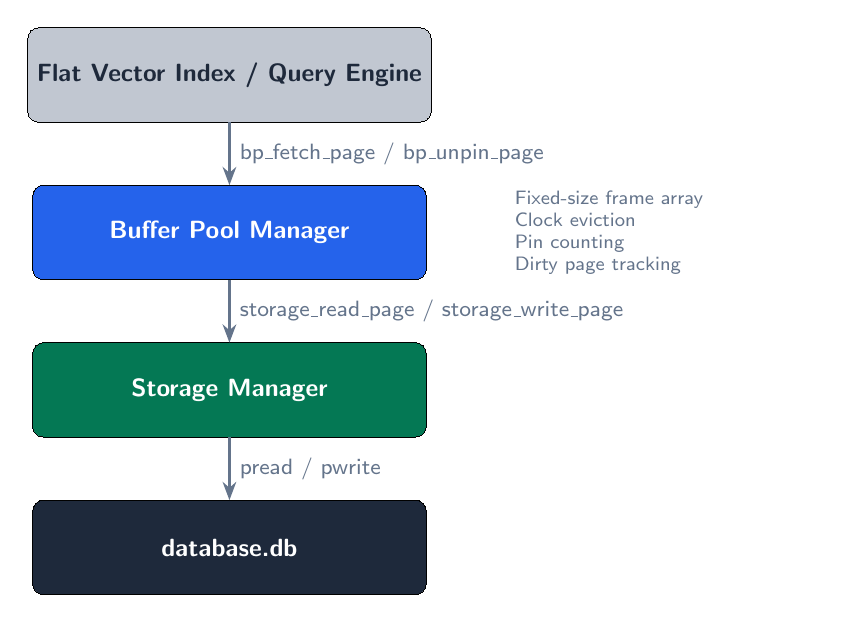
\begin{tikzpicture}[
    box/.style={draw, rounded corners=4pt, minimum width=5cm, minimum height=1.2cm,
                text=white, font=\sffamily\small\bfseries, line width=0},
    arr/.style={-Stealth, thick, proto-gray},
    lbl/.style={font=\sffamily\footnotesize, text=proto-gray},
]
    % Layers
    \node[box, fill=proto-gray!40, text=proto-dark] (upper) at (0, 6) {Flat Vector Index / Query Engine};
    \node[box, fill=proto-blue]                     (bp)    at (0, 4) {Buffer Pool Manager};
    \node[box, fill=proto-green!80!black]           (sm)    at (0, 2) {Storage Manager};
    \node[box, fill=proto-dark]                     (disk)  at (0, 0) {database.db};

    % Arrows
    \draw[arr] (upper) -- (bp)   node[midway, right, lbl] {bp\_fetch\_page / bp\_unpin\_page};
    \draw[arr] (bp)    -- (sm)   node[midway, right, lbl] {storage\_read\_page / storage\_write\_page};
    \draw[arr] (sm)    -- (disk) node[midway, right, lbl] {pread / pwrite};

    % Side note
    \node[anchor=west, font=\sffamily\scriptsize, text=proto-gray, text width=4cm]
        at (3.5, 4) {Fixed-size frame array\\Clock eviction\\Pin counting\\Dirty page tracking};
\end{tikzpicture}
\end{center}

The key contract: \textbf{no layer above the buffer pool touches the storage
manager directly.} All page I/O flows through \texttt{bp\_fetch\_page} and
\texttt{bp\_unpin\_page}. This gives the buffer pool full control over what's
in memory and when disk writes happen.


% ── 3.2 Frame Array ──────────────────────────────────────────────────────────
\section{Frame Array}

The buffer pool manages a fixed-size array of \texttt{Page} structs called
\textbf{frames}. The number of frames is set at initialization and does not
change.

\begin{lstlisting}
typedef struct {
  Page *frames;
  page_id_t *pt_keys;
  int32_t *pt_vals;
  uint32_t pt_capacity;
  bool *ref_bits;
  uint32_t clock_hand;
  uint32_t num_frames;
  StorageManager *sm;
} BufferPool;
\end{lstlisting}

Each frame holds one page's data. The transient fields on the \texttt{Page}
struct---\texttt{pin\_count} and \texttt{is\_dirty}---are now actively managed
by the buffer pool rather than being unused placeholders.

\begin{itemize}[itemsep=4pt]
    \item \textbf{pin\_count} --- Incremented on every \texttt{bp\_fetch\_page},
          decremented on every \texttt{bp\_unpin\_page}. A frame with
          pin\_count $> 0$ is ``pinned'' and cannot be evicted.
    \item \textbf{is\_dirty} --- Set when the caller passes
          \texttt{is\_dirty = true} to \texttt{bp\_unpin\_page}. A dirty
          frame must be flushed to disk before its frame can be reused.
\end{itemize}


% ── 3.3 Page Table ───────────────────────────────────────────────────────────
\section{Page Table}

The buffer pool needs a fast mapping from \texttt{page\_id} to frame index.
This is the \textbf{page table}---an open-addressing hash map with linear
probing.

\begin{table}[h]
\centering
\begin{tabularx}{\textwidth}{lXX}
\toprule
\textbf{Approach} & \textbf{Pro} & \textbf{Con} \\
\midrule
\textbf{Open addressing (ours)} &
    No heap allocations per lookup, cache-friendly linear memory access,
    simple implementation &
    Needs tombstone handling on delete (we re-insert displaced entries),
    load factor must stay low \\
\addlinespace
Chained hash map &
    Handles high load factors gracefully, simpler deletion &
    One \texttt{malloc} per entry, pointer chasing is cache-unfriendly \\
\addlinespace
Direct array &
    O(1) with no hashing &
    Size must equal max page\_id, wastes memory for sparse ID spaces \\
\bottomrule
\end{tabularx}
\caption{Page table implementation strategies}
\end{table}

We use \textbf{Fibonacci hashing}\footnote{Knuth, D.~E.
\textit{The Art of Computer Programming}, Vol.~3, Section 6.4.} to
distribute sequential page IDs well:

\begin{lstlisting}
static uint32_t hash_page_id(page_id_t id, uint32_t capacity) {
  uint32_t h = id * 2654435769u;
  return h & (capacity - 1);
}
\end{lstlisting}

The magic constant \texttt{2654435769} is $\lfloor 2^{32} / \varphi \rfloor$
where $\varphi = \frac{1+\sqrt{5}}{2}$ (the golden ratio). This spreads
consecutive integers across the table far better than modular hashing.

The table capacity is always a power of two ($\geq 2 \times
\texttt{num\_frames}$) to keep the load factor below 0.5 and allow
bitwise-AND masking instead of modulo division.

\subsection{Deletion: Backward Shift}

Deleting from an open-addressing table is tricky. Simply zeroing a slot
can break the probe chain for other entries that hashed to earlier slots.
Our approach: after removing an entry, re-insert all subsequent entries in
the same probe cluster.

\begin{lstlisting}
uint32_t next = (slot + 1) & (bp->pt_capacity - 1);
while (bp->pt_keys[next] != BP_EMPTY_SLOT) {
  page_id_t k = bp->pt_keys[next];
  int32_t v = bp->pt_vals[next];
  bp->pt_keys[next] = BP_EMPTY_SLOT;
  bp->pt_vals[next] = -1;
  pt_insert(bp, k, v);
  next = (next + 1) & (bp->pt_capacity - 1);
}
\end{lstlisting}

This is equivalent to the ``backward shift deletion'' technique described
in Knuth's TAOCP Vol.~3, Algorithm R.


% ── 3.4 Clock Eviction ──────────────────────────────────────────────────────
\section{Clock (Second-Chance) Eviction}

When all frames are occupied and a new page is needed, the buffer pool must
\textbf{evict} a page. We use the \textbf{clock algorithm}, also known as
second-chance---a practical approximation of LRU.

\begin{center}
\begin{tikzpicture}[
    frame/.style={draw, rounded corners=2pt, minimum width=1.5cm,
                  minimum height=1cm, font=\sffamily\scriptsize},
    arr/.style={-Stealth, very thick, proto-blue},
]
    % Clock circle
    \foreach \i/\ref/\pin in {0/1/0, 1/0/0, 2/1/1, 3/0/0, 4/1/0, 5/0/0} {
        \pgfmathsetmacro{\angle}{90 - \i * 60}
        \node[frame,
              fill=\ifnum\pin=1 proto-red!15\else\ifnum\ref=1 proto-blue!15\else proto-green!15\fi\fi]
            (f\i) at (\angle:2.8cm) {F\i\\[-2pt]ref=\ref\ifnum\pin=1\\pin\fi};
    }

    % Clock hand pointing at frame 1
    \draw[arr] (0,0) -- (f1);

    % Legend
    \node[anchor=north west, font=\sffamily\scriptsize, text=proto-dark,
          text width=5cm] at (4, 2.5) {
        \textcolor{proto-green!60!black}{$\blacksquare$} ref=0, unpinned $\to$ \textbf{evict}\\
        \textcolor{proto-blue}{$\blacksquare$} ref=1, unpinned $\to$ clear, skip\\
        \textcolor{proto-red}{$\blacksquare$} pinned $\to$ always skip
    };

    % Center label
    \node[font=\sffamily\small\bfseries, text=proto-dark] at (0, 0) {Clock};
\end{tikzpicture}
\end{center}

The algorithm:
\begin{enumerate}[itemsep=2pt]
    \item Start at \texttt{clock\_hand}.
    \item If the frame is pinned, skip it.
    \item If \texttt{ref\_bit = 1}, clear it to 0 (second chance) and advance.
    \item If \texttt{ref\_bit = 0}, this is the victim. If dirty, flush to disk
          first.
    \item Advance the hand and repeat. After $2 \times \texttt{num\_frames}$
          sweeps without finding a victim, all frames are pinned---return
          \texttt{NULL}.
\end{enumerate}

\begin{table}[h]
\centering
\begin{tabularx}{\textwidth}{lXX}
\toprule
\textbf{Policy} & \textbf{Pro} & \textbf{Con} \\
\midrule
\textbf{Clock (ours)} &
    O(1) amortized, no linked list overhead, approximates LRU well &
    Not true LRU---recently used pages may still be evicted if
    ref\_bit was cleared on a prior sweep \\
\addlinespace
LRU (linked list) &
    Exact LRU ordering, optimal for most workloads &
    Requires a doubly-linked list + hash map, more pointer chasing,
    higher constant overhead \\
\addlinespace
LRU-K &
    Handles scan-resistant workloads better than plain LRU &
    Significantly more complex (track K-th most recent access
    timestamp per page) \\
\bottomrule
\end{tabularx}
\caption{Buffer pool eviction policy comparison}
\end{table}

Clock was chosen because it's what BusTub uses in the CMU 15-445 Project 1,
and it gives us near-LRU behavior with a much simpler implementation---a
single array of booleans and one integer for the hand position.


% ── 3.5 API ──────────────────────────────────────────────────────────────────
\section{Public API}

\begin{lstlisting}
int bp_init(BufferPool *bp, StorageManager *sm, uint32_t num_frames);
void bp_destroy(BufferPool *bp);

Page *bp_fetch_page(BufferPool *bp, page_id_t page_id);
int bp_unpin_page(BufferPool *bp, page_id_t page_id, bool is_dirty);
int bp_flush_page(BufferPool *bp, page_id_t page_id);
int bp_flush_all(BufferPool *bp);

Page *bp_new_page(BufferPool *bp, page_id_t *out);
int bp_delete_page(BufferPool *bp, page_id_t page_id);
\end{lstlisting}

\subsection{Fetch / Unpin Lifecycle}

Every \texttt{bp\_fetch\_page} must be paired with a \texttt{bp\_unpin\_page}.
This is the ``acquire/release'' pattern:

\begin{lstlisting}
Page *p = bp_fetch_page(&bp, page_id);  // pin_count++
// ... read or modify p->data ...
bp_unpin_page(&bp, page_id, true);      // pin_count--, mark dirty
\end{lstlisting}

Forgetting to unpin is a resource leak---the frame will never be evictable,
eventually exhausting the pool. This is the buffer pool equivalent of a
memory leak.

\subsection{New Page / Delete Page}

\texttt{bp\_new\_page} combines \texttt{storage\_allocate\_page} with loading
the fresh page into a frame. The new page is returned pinned and dirty (since
it hasn't been written to disk yet in its initialized state).

\texttt{bp\_delete\_page} refuses to delete a pinned page (returns -1). On
success, it removes the page from the frame array and calls
\texttt{storage\_deallocate\_page} to return it to the free list.

\subsection{Flush}

\texttt{bp\_flush\_page} forces a single page to disk immediately.
\texttt{bp\_flush\_all} writes all dirty pages. \texttt{bp\_destroy} calls
\texttt{bp\_flush\_all} implicitly before freeing memory, so dirty pages are
never lost on clean shutdown.


% ── 3.6 Concurrency Control ──────────────────────────────────────────────────
\section{Concurrency Control}

To support concurrent database operations (such as parallel index building or query execution), the Buffer Pool Manager is fully thread-safe. It uses a two-tier latching strategy, similar to real DBMS engines like PostgreSQL and InnoDB:

\begin{enumerate}[itemsep=4pt]
    \item \textbf{Global Buffer Pool Latch (\texttt{pthread\_mutex\_t})}: A single mutex protects the internal metadata of the buffer pool, including the page table, the frame array, the clock hand, and the \texttt{is\_dirty} flags. Any operation that changes this state (e.g., fetching a new page, running eviction, pinning/unpinning) must acquire this latch.
    \item \textbf{Page Latches (\texttt{pthread\_rwlock\_t})}: Each \texttt{Page} struct contains its own reader-writer latch to protect its \texttt{data} buffer. Once a thread has successfully pinned a page via \texttt{bp\_fetch\_page}, it must acquire the page's \texttt{rwlatch} (via \texttt{page\_rlock} or \texttt{page\_wlock}) before reading or modifying the records inside it.
\end{enumerate}

This separation ensures that multiple threads can concurrently read or write to \textit{different} pages in memory without blocking each other, while still guaranteeing that the buffer pool's core data structures cannot be corrupted by race conditions.


% ── 3.7 References ───────────────────────────────────────────────────────────
\section{References}

\begin{enumerate}[itemsep=6pt]
    \item \textbf{CMU 15-445: Buffer Pools} (Andy Pavlo)\\
          \url{https://15445.courses.cs.cmu.edu/}\\
          Lectures 5--6 cover buffer pool design, eviction policies, and
          the pin/unpin contract. Project 1 is a direct implementation
          of this component.

    \item \textbf{Database Internals} (Alex Petrov, O'Reilly 2019)\\
          Chapter 5 (Transaction Processing and Recovery) discusses
          buffer management, page replacement, and write-ahead logging.

    \item \textbf{The Art of Computer Programming, Vol. 3}
          (Donald E. Knuth)\\
          Section 6.4 covers hashing techniques including Fibonacci
          hashing. Algorithm R covers open-addressing deletion.

    \item \textbf{BusTub} (CMU Database Group)\\
          \url{https://github.com/cmu-db/bustub}\\
          The \texttt{BufferPoolManager} and \texttt{ClockReplacer}
          classes directly informed our implementation.

    \item \textbf{Operating System Concepts, 10th ed.}
          (Silberschatz, Galvin \& Gagne)\\
          Chapter 10 (Virtual Memory) describes the clock algorithm
          in the context of OS page replacement---the same algorithm
          we apply here to database pages.
\end{enumerate}


% ══════════════════════════════════════════════════════════════════════════════
\chapter{Flat Vector Index}
% ══════════════════════════════════════════════════════════════════════════════

With the buffer pool in place, we can build something on top of it. The first
index in ProtoDB is a \textbf{flat vector index}---a brute-force nearest
neighbor search over dense float vectors. It's the simplest possible vector
index: store every vector, and on query, compare against all of them.

This is intentionally boring. The goal is to get the foundational plumbing
right---vector page layout, distance functions, the top-k result heap, and
the I/O path through the buffer pool---so that a future approximate index
(HNSW) can reuse all of it.


% ── 4.1 Architecture ─────────────────────────────────────────────────────────
\section{Architecture Overview}

The flat index sits on top of the buffer pool and introduces four new
components:

\begin{center}
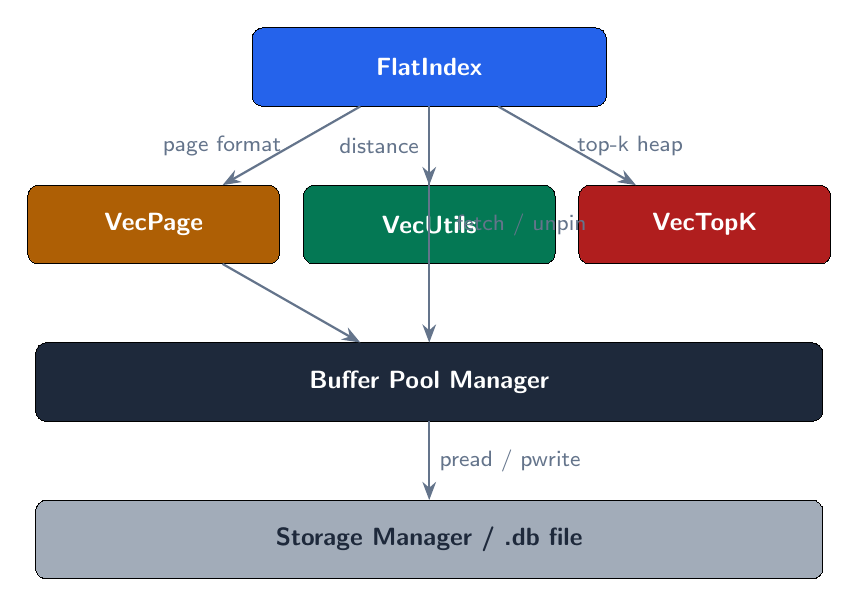
\begin{tikzpicture}[
    box/.style={draw, rounded corners=4pt, minimum width=4.5cm, minimum height=1cm,
                text=white, font=\sffamily\small\bfseries, line width=0},
    arr/.style={-Stealth, thick, proto-gray},
    lbl/.style={font=\sffamily\footnotesize, text=proto-gray},
]
    % Top level
    \node[box, fill=proto-blue] (flat) at (0, 6) {FlatIndex};

    % Middle components
    \node[box, fill=proto-orange!80!black, minimum width=3.2cm] (vp) at (-3.5, 4)
        {VecPage};
    \node[box, fill=proto-green!80!black, minimum width=3.2cm] (vu) at (0, 4)
        {VecUtils};
    \node[box, fill=proto-red!80!black, minimum width=3.2cm] (tk) at (3.5, 4)
        {VecTopK};

    % Buffer pool
    \node[box, fill=proto-dark, minimum width=10cm] (bp) at (0, 2)
        {Buffer Pool Manager};

    % Storage
    \node[box, fill=proto-gray!60, text=proto-dark, minimum width=10cm] (sm) at (0, 0)
        {Storage Manager / .db file};

    % Arrows
    \draw[arr] (flat) -- (vp)  node[midway, left,  lbl] {page format};
    \draw[arr] (flat) -- (vu)  node[midway, left,  lbl] {distance};
    \draw[arr] (flat) -- (tk)  node[midway, right, lbl] {top-k heap};
    \draw[arr] (vp)  -- (bp);
    \draw[arr] (flat) -- (bp)  node[midway, right, lbl, xshift=6pt] {fetch / unpin};
    \draw[arr] (bp)  -- (sm)   node[midway, right, lbl] {pread / pwrite};
\end{tikzpicture}
\end{center}

\begin{itemize}[itemsep=4pt]
    \item \textbf{VecUtils} --- Pure-compute distance functions (L2, cosine,
          inner product) and vector normalization. No I/O dependencies.
    \item \textbf{VecTopK} --- A max-heap that tracks the $k$ smallest
          distances seen during a scan.
    \item \textbf{VecPage} --- Defines how vectors are packed into 8 KB pages
          using \texttt{PAGE\_TYPE\_VECTOR}.
    \item \textbf{FlatIndex} --- Manages a growable list of vector pages and
          orchestrates brute-force scans.
\end{itemize}

Each component is in its own \texttt{.h/.c} pair under \texttt{src/index/}.
They have a clean dependency order: VecUtils and VecTopK are leaf modules
with no cross-dependencies, VecPage depends only on the existing page layer,
and FlatIndex ties everything together.


% ── 4.2 Vector Page Layout ───────────────────────────────────────────────────
\section{Vector Page Layout}

Generic data pages use a slotted layout with variable-length records. Vector
pages are different: every vector has the same dimensionality, so we use a
\textbf{fixed-width} layout with no slot array.

\begin{center}
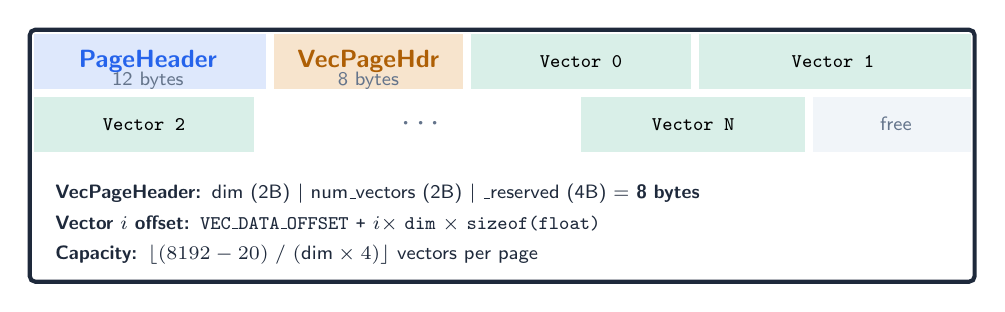
\begin{tikzpicture}[
    cell/.style={draw, minimum height=0.8cm, font=\ttfamily\scriptsize, anchor=west},
]
    \def\pw{12}
    \def\ph{0.8}

    % Page outline
    \draw[proto-dark, line width=1.5pt, rounded corners=2pt] (0,0) rectangle (\pw, -4*\ph);

    % PageHeader
    \fill[proto-blue!15] (0.05, -0.05) rectangle (3, -\ph+0.05);
    \node[font=\sffamily\small\bfseries, text=proto-blue] at (1.5, -\ph/2)
        {PageHeader};
    \node[font=\sffamily\scriptsize, text=proto-gray] at (1.5, -\ph/2-0.25)
        {12 bytes};

    % VecPageHeader
    \fill[proto-orange!20] (3.1, -0.05) rectangle (5.5, -\ph+0.05);
    \node[font=\sffamily\small\bfseries, text=proto-orange!80!black] at (4.3, -\ph/2)
        {VecPageHdr};
    \node[font=\sffamily\scriptsize, text=proto-gray] at (4.3, -\ph/2-0.25)
        {8 bytes};

    % Vectors
    \fill[proto-green!15] (5.6, -0.05) rectangle (8.4, -\ph+0.05);
    \node[font=\ttfamily\scriptsize] at (7.0, -\ph/2) {Vector 0};

    \fill[proto-green!15] (8.5, -0.05) rectangle (\pw-0.05, -\ph+0.05);
    \node[font=\ttfamily\scriptsize] at (10.2, -\ph/2) {Vector 1};

    \fill[proto-green!15] (0.05, -\ph-0.05) rectangle (2.85, -2*\ph+0.05);
    \node[font=\ttfamily\scriptsize] at (1.45, -1.5*\ph) {Vector 2};

    \node[font=\sffamily\large, text=proto-gray] at (5, -1.5*\ph) {$\cdots$};

    \fill[proto-green!15] (7, -\ph-0.05) rectangle (9.85, -2*\ph+0.05);
    \node[font=\ttfamily\scriptsize] at (8.425, -1.5*\ph) {Vector N};

    % Free space
    \fill[proto-light] (9.95, -\ph-0.05) rectangle (\pw-0.05, -2*\ph+0.05);
    \node[font=\sffamily\scriptsize, text=proto-gray] at (11, -1.5*\ph) {free};

    % Details
    \node[anchor=north west, font=\sffamily\scriptsize, text=proto-dark,
          text width=11.5cm] at (0.2, -2.3*\ph) {
        \textbf{VecPageHeader:} dim (2B) $\mid$ num\_vectors (2B) $\mid$
        \_reserved (4B) = \textbf{8 bytes}\\[3pt]
        \textbf{Vector $i$ offset:} \texttt{VEC\_DATA\_OFFSET + $i \times$ dim $\times$ sizeof(float)}\\[3pt]
        \textbf{Capacity:} $\lfloor(8192 - 20) \;/\; (\text{dim} \times 4)\rfloor$ vectors per page
    };
\end{tikzpicture}
\end{center}

\subsection{Why Fixed-Width?}

\begin{table}[h]
\centering
\begin{tabularx}{\textwidth}{lXX}
\toprule
\textbf{Approach} & \textbf{Advantage} & \textbf{Disadvantage} \\
\midrule
\textbf{Fixed-width (ours)} &
    O(1) random access by index, no slot array overhead, cache-friendly
    sequential scan, zero-copy reads via pointer into page data &
    All vectors must share the same dimension; no mixed-dim pages \\
\addlinespace
Slotted page (reuse existing) &
    Works for variable-length data, already implemented &
    4-byte slot overhead per record, indirect access,
    compaction complexity for data that never varies in size \\
\bottomrule
\end{tabularx}
\caption{Vector page format tradeoff}
\end{table}

Since all vectors in an index have the same dimension, fixed-width is
strictly better. We get deterministic offset math and zero bookkeeping.

\subsection{Capacity Examples}

With an 8 KB page, 12-byte \texttt{PageHeader}, and 8-byte
\texttt{VecPageHeader}, the usable space is $8192 - 20 = 8172$ bytes.

\begin{table}[h]
\centering
\begin{tabular}{rrrr}
\toprule
\textbf{Dimension} & \textbf{Bytes/Vector} & \textbf{Vectors/Page} & \textbf{Use Case} \\
\midrule
4   & 16   & 510 & Toy / testing \\
128 & 512  & 15  & Word2Vec, GloVe \\
384 & 1536 & 5   & all-MiniLM-L6-v2 \\
768 & 3072 & 2   & OpenAI text-embedding-3-small \\
1024 & 4096 & 1  & Large embeddings \\
\bottomrule
\end{tabular}
\caption{Vectors per page for common embedding dimensions}
\end{table}

For high-dimensional embeddings (768+), only a few vectors fit per page,
which means more I/O during a flat scan. This is expected---and is exactly
why approximate indexes like HNSW exist.


% ── 4.3 Distance Functions ───────────────────────────────────────────────────
\section{Distance Functions}

The index supports three distance metrics. All are implemented as
straightforward loops in \texttt{vec\_utils.c}---no SIMD for now.

\subsection{Squared Euclidean (L2\textsuperscript{2})}

\[
d_{L2^2}(\mathbf{a}, \mathbf{b}) = \sum_{i=1}^{d} (a_i - b_i)^2
\]

We use the \textit{squared} distance during the scan to avoid a
\texttt{sqrtf} per comparison. Since $\sqrt{\cdot}$ is monotonic, the
ranking is identical. A full \texttt{vec\_l2\_distance} (with sqrt) is
available for callers that need the true distance.

\subsection{Cosine Distance}

\[
d_{\cos}(\mathbf{a}, \mathbf{b}) = 1 - \frac{\mathbf{a} \cdot \mathbf{b}}
    {\|\mathbf{a}\| \; \|\mathbf{b}\|}
\]

Range: $[0, 2]$. A distance of 0 means identical direction. We clamp the
cosine similarity to $[-1, 1]$ to guard against floating-point drift, and
return 1.0 for zero-magnitude vectors to avoid division by zero.

\subsection{Inner Product Distance}

\[
d_{IP}(\mathbf{a}, \mathbf{b}) = -(\mathbf{a} \cdot \mathbf{b})
\]

The negation ensures that \textit{higher} dot products produce
\textit{smaller} distances, so the top-k heap's ``smallest distance wins''
convention works uniformly across all metrics. This is the same trick used by
Faiss\footnote{Johnson, J., Douze, M., \& J{\'e}gou, H. \textit{Billion-scale
similarity search with GPUs.} IEEE Transactions on Big Data, 2019.
\url{https://github.com/facebookresearch/faiss}} and pgvector.

\subsection{Why These Three?}

These are the three metrics supported by essentially every vector database
(pgvector\footnote{\url{https://github.com/pgvector/pgvector}},
Pinecone, Milvus, Qdrant). L2 is the geometric default. Cosine is standard
for text embeddings (where magnitude is irrelevant). Inner product is used
for maximum inner product search (MIPS), common in recommendation systems.


% ── 4.4 Top-K Heap ───────────────────────────────────────────────────────────
\section{Top-K Heap}

During a scan, we need to track the $k$ nearest vectors seen so far. A
na{\"i}ve approach (collect all distances, sort, take top $k$) would be
$O(n \log n)$ for $n$ vectors. Instead, we use a \textbf{max-heap} of size
$k$, giving us $O(n \log k)$.

\begin{center}
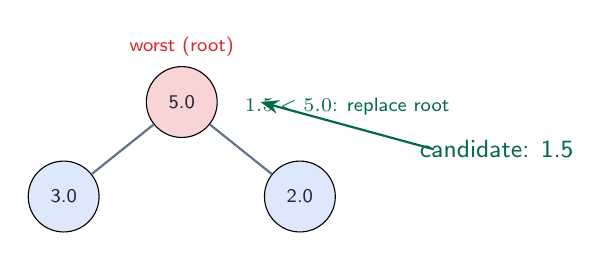
\begin{tikzpicture}[
    node/.style={draw, circle, minimum size=0.9cm, font=\sffamily\scriptsize,
                 fill=proto-blue!15, text=proto-dark},
    arr/.style={-Stealth, thick, proto-gray},
]
    % Heap nodes
    \node[node, fill=proto-red!20] (root) at (0, 0) {5.0};
    \node[node] (l)    at (-1.5, -1.2) {3.0};
    \node[node] (r)    at (1.5, -1.2)  {2.0};

    \draw[proto-gray, thick] (root) -- (l);
    \draw[proto-gray, thick] (root) -- (r);

    % Labels
    \node[font=\sffamily\scriptsize, text=proto-red, anchor=south] at (root.north)
        {worst (root)};

    % Candidate
    \node[font=\sffamily\small, text=proto-green!70!black] at (4, -0.6)
        {candidate: 1.5};
    \draw[arr, proto-green!70!black] (3.2, -0.6) -- (1, 0)
        node[midway, above, font=\sffamily\scriptsize, text=proto-green!70!black]
        {$1.5 < 5.0$: replace root};
\end{tikzpicture}
\end{center}

The invariant: the heap root is always the \textit{largest} distance in the
current top-$k$ set. When a new candidate arrives:

\begin{itemize}[itemsep=2pt]
    \item If the heap has fewer than $k$ items, insert unconditionally.
    \item If the candidate's distance $\geq$ root distance, skip it.
    \item Otherwise, replace the root and sift down.
\end{itemize}

After the scan, a single \texttt{qsort} puts the results in ascending
distance order.


% ── 4.5 Flat Index ───────────────────────────────────────────────────────────
\section{Flat Index}

The \texttt{FlatIndex} struct ties everything together:

\begin{lstlisting}
typedef struct {
    BufferPool        *bp;
    uint16_t           dim;
    VecDistanceMetric  metric;
    page_id_t         *page_ids;
    uint32_t           num_pages;
    uint32_t           page_cap;
    uint32_t           total_vectors;
} FlatIndex;
\end{lstlisting}

The \texttt{page\_ids} array is a growable dynamic array (starting at
capacity 16, doubled on overflow) that tracks which pages belong to this
index. This is managed entirely in memory---there's no on-disk index
metadata page yet.

\subsection{Insert Path}

\begin{center}
\begin{tikzpicture}[
    node distance=1cm,
    process/.style={draw, rounded corners=3pt, fill=proto-green!10, text=proto-dark,
                    font=\sffamily\scriptsize, minimum width=3.5cm, minimum height=0.6cm},
    decision/.style={diamond, draw, fill=proto-blue!10, text=proto-dark,
                     font=\sffamily\scriptsize, aspect=2.5, inner sep=1pt},
    arr/.style={-Stealth, thick, proto-gray},
]
    \node[process] (fetch) {Fetch last page via buffer pool};
    \node[decision, below=of fetch] (full) {Page full?};
    \node[process, below left=1cm and 1.5cm of full] (append) {Append vector to page\\Mark dirty, unpin};
    \node[process, below right=1cm and 1.5cm of full] (alloc) {Unpin last page\\Allocate new vector page};
    \node[process, below=2.5cm of full] (done) {Return (page\_id, slot)};

    \draw[arr] (fetch) -- (full);
    \draw[arr] (full) -| node[near start, above, font=\sffamily\scriptsize] {no} (append);
    \draw[arr] (full) -| node[near start, above, font=\sffamily\scriptsize] {yes} (alloc);
    \draw[arr] (append) |- (done);
    \draw[arr] (alloc) |- ([yshift=-0.3cm]alloc.south) -| ([xshift=-1cm]done.north) -- (done);
\end{tikzpicture}
\end{center}

Inserts always go to the last page. When it fills up, we call
\texttt{bp\_new\_page} to allocate a fresh vector page, initialize it with
\texttt{vec\_page\_init}, and append the \texttt{page\_id} to our tracking
array. The caller gets back a \texttt{(page\_id, slot\_index)} pair
identifying the stored vector.


\subsection{Search Path}

Search is a full sequential scan:

\begin{lstlisting}
for each page_id in idx->page_ids:
    page = bp_fetch_page(bp, page_id)
    for i in 0..vec_page_count(page):
        vec = vec_page_get(page, i)   // zero-copy pointer
        dist = distance_fn(query, vec, dim)
        vec_topk_push(&topk, page_id, i, dist)
    bp_unpin_page(bp, page_id, false) // read-only, not dirty
vec_topk_sort(&topk)
\end{lstlisting}

Every vector is compared against the query. The top-k heap prunes
candidates that can't improve the result set. Pages are fetched and
unpinned one at a time, so the buffer pool's clock eviction handles memory
pressure naturally---we never need more than one frame pinned at a time
during the scan.


\subsection{Deletion}

Vectors can be marked as deleted using a tombstone mechanism. 
The \texttt{VecPageHeader} includes a 128-byte \texttt{deleted\_bitmap} which tracks up to 1024 vectors per page.
When \texttt{flat\_index\_delete} is called, the index locates the vector's page and slot, and sets the corresponding bit in the bitmap. 
The search path is updated to check this bitmap via \texttt{vec_page_is_deleted(page, i)} and skips vectors that have been marked as deleted. This avoids costly in-place compaction while safely removing vectors from search results.

\subsection{Complexity}

\begin{table}[h]
\centering
\begin{tabular}{lll}
\toprule
\textbf{Operation} & \textbf{Time} & \textbf{I/O} \\
\midrule
Insert     & $O(1)$ amortized & 1 page fetch + possible page allocation \\
Search     & $O(n \cdot d + n \log k)$ & 1 fetch per vector page \\
\bottomrule
\end{tabular}
\caption{Flat index operation costs ($n$ = vectors, $d$ = dimension, $k$ = result size)}
\end{table}

Search is $O(n)$ in the number of stored vectors---that's the price of
exactness. For small datasets (up to tens of thousands of vectors), this
is perfectly acceptable. Beyond that, you need an approximate index.


% ── 4.6 What This Gets Us ───────────────────────────────────────────────────
\section{What This Gets Us}

The flat index is not the end goal. It's the \textbf{foundation} that a
future HNSW index will build on:

\begin{itemize}[itemsep=4pt]
    \item \textbf{Vector page format} --- HNSW will store vectors on the same
          \texttt{PAGE\_TYPE\_VECTOR} pages. The packing/unpacking code is
          already done.
    \item \textbf{Distance functions} --- Shared between flat scan and graph
          traversal. Adding SIMD later benefits both.
    \item \textbf{Top-k heap} --- The same heap drives HNSW's greedy
          search through graph layers.
    \item \textbf{Correct baseline} --- We can validate HNSW's approximate
          results against the flat index's exact results. If the flat
          index says vector \#42 is the nearest neighbor, HNSW should
          return it too (at least most of the time).
\end{itemize}


% ── 4.7 References ───────────────────────────────────────────────────────────
\section{References}

\begin{enumerate}[itemsep=6pt]
    \item \textbf{pgvector} (Andrew Kane)\\
          \url{https://github.com/pgvector/pgvector}\\
          PostgreSQL extension for vector similarity search. Its flat
          index (sequential scan with distance operators) is the direct
          inspiration for our approach.

    \item \textbf{Faiss} (Facebook AI Research)\\
          Johnson, J., Douze, M., \& J{\'e}gou, H. \textit{Billion-scale
          similarity search with GPUs.} IEEE Transactions on Big Data, 2019.\\
          \url{https://github.com/facebookresearch/faiss}\\
          The \texttt{IndexFlat} class is the canonical flat vector index.
          Our negative inner product convention matches theirs.

    \item \textbf{CMU 15-445: Database Systems} (Andy Pavlo)\\
          \url{https://15445.courses.cs.cmu.edu/}\\
          The buffer pool contract (fetch/unpin) that the flat index
          builds on.

    \item \textbf{Database Internals} (Alex Petrov, O'Reilly 2019)\\
          Chapter 7 covers B-tree and LSM index structures. The flat
          index is simpler than both, but the page management patterns
          are the same.

    \item \textbf{``Efficient and Robust Approximate Nearest Neighbor
          Search Using Hierarchical Navigable Small World Graphs''}
          (Malkov \& Yashunin, 2018)\\
          \url{https://arxiv.org/abs/1603.09320}\\
          The HNSW paper---where we're headed next.
\end{enumerate}



% ═════════════════════════════════════════════════════════════════════════════
%  CHAPTER 5: INVERTED FILE (IVF) INDEX
% ═════════════════════════════════════════════════════════════════════════════
\chapter{Inverted File (IVF) Index}

\section{Overview}
While the Flat Index provides exact nearest neighbor search, its $O(n)$ search complexity becomes a bottleneck for larger datasets. To address this, ProtoDB implements an Inverted File (IVF) Index, a classic approximate nearest neighbor (ANN) algorithm.

\section{Architecture}
The IVF index partitions the vector space into \texttt{nlist} Voronoi cells, each defined by a centroid. 
Vectors are assigned to the cell of their nearest centroid. During search, the query is compared against all centroids, and only the vectors in the \texttt{nprobe} closest cells are scanned.

\subsection{Centroid Training}
Before inserting vectors, the index must be trained. A subset of vectors is used to compute the centroids using K-Means clustering. 

\subsection{Partitions}
Each centroid has an associated partition, which is essentially a dynamically sized array of vector page IDs. Vectors are inserted into the pages of their respective partition. 

\section{Performance}
By tuning \texttt{nlist} and \texttt{nprobe}, the user trades off recall accuracy for search speed. In our benchmarks, an IVF index with \texttt{nlist=32} and \texttt{nprobe=4} scans only ~12\% of the dataset, increasing search throughput from ~1,300 QPS (Flat) to over ~19,500 QPS on 128-dimensional vectors.

% ═════════════════════════════════════════════════════════════════════════════
%  CHAPTER 6: PERSISTENCE AND STREAM PAGES
% ═════════════════════════════════════════════════════════════════════════════
\chapter{Persistence and Stream Pages}

\section{The Need for Persistence}
Indexes in ProtoDB originally built their metadata (e.g., page ID arrays for Flat, centroids and partition arrays for IVF) strictly in memory. While the underlying vector pages were written to disk via the buffer pool, the structural links to find them would be lost on restart.

\section{Stream Pages}
To serialize dynamically sized arrays (like \texttt{idx->page\_ids}), we introduced \texttt{PAGE\_TYPE\_STREAM}.
A Stream Page allows storing arbitrary byte streams across multiple linked pages on disk.
The \texttt{StreamPageHeader} contains a \texttt{next\_page\_id} and \texttt{data\_size}.
This acts as a linked list of pages, enabling us to serialize index metadata that exceeds the 8KB limit of a single page.

\section{Index Serialization}
Each index type implements a \texttt{save} and \texttt{load} routine:
\begin{itemize}
    \item \textbf{Flat Index}: Serializes a \texttt{FlatIndexMeta} header followed by the array of vector page IDs.
    \item \textbf{IVF Index}: Iterates through all partitions, saves them using stream pages, and then serializes the \texttt{IvfIndexMeta}, centroids, and the array of partition root page IDs.
\end{itemize}

The root page ID of the main index stream is stored in the \texttt{MetaPageHeader} (page 0), allowing ProtoDB to seamlessly rebuild the entire database state upon restart.


\end{document}
